%\documentclass[handout,xcolor=pdftex,dvipsnames,table]{beamer}
%\documentclass[draft]{beamer}
%\documentclass[notesonly]{beamer}
%\documentclass[notes]{beamer}
\documentclass[aspectratio=169, xcolor=table]{beamer}\usepackage[]{graphicx}\usepackage[]{color}
%% maxwidth is the original width if it is less than linewidth
%% otherwise use linewidth (to make sure the graphics do not exceed the margin)
\makeatletter
\def\maxwidth{ %
  \ifdim\Gin@nat@width>\linewidth
    \linewidth
  \else
    \Gin@nat@width
  \fi
}
\makeatother

\definecolor{fgcolor}{rgb}{0.345, 0.345, 0.345}
\newcommand{\hlnum}[1]{\textcolor[rgb]{0.686,0.059,0.569}{#1}}%
\newcommand{\hlstr}[1]{\textcolor[rgb]{0.192,0.494,0.8}{#1}}%
\newcommand{\hlcom}[1]{\textcolor[rgb]{0.678,0.584,0.686}{\textit{#1}}}%
\newcommand{\hlopt}[1]{\textcolor[rgb]{0,0,0}{#1}}%
\newcommand{\hlstd}[1]{\textcolor[rgb]{0.345,0.345,0.345}{#1}}%
\newcommand{\hlkwa}[1]{\textcolor[rgb]{0.161,0.373,0.58}{\textbf{#1}}}%
\newcommand{\hlkwb}[1]{\textcolor[rgb]{0.69,0.353,0.396}{#1}}%
\newcommand{\hlkwc}[1]{\textcolor[rgb]{0.333,0.667,0.333}{#1}}%
\newcommand{\hlkwd}[1]{\textcolor[rgb]{0.737,0.353,0.396}{\textbf{#1}}}%
\let\hlipl\hlkwb

\usepackage{framed}
\makeatletter
\newenvironment{kframe}{%
 \def\at@end@of@kframe{}%
 \ifinner\ifhmode%
  \def\at@end@of@kframe{\end{minipage}}%
  \begin{minipage}{\columnwidth}%
 \fi\fi%
 \def\FrameCommand##1{\hskip\@totalleftmargin \hskip-\fboxsep
 \colorbox{shadecolor}{##1}\hskip-\fboxsep
     % There is no \\@totalrightmargin, so:
     \hskip-\linewidth \hskip-\@totalleftmargin \hskip\columnwidth}%
 \MakeFramed {\advance\hsize-\width
   \@totalleftmargin\z@ \linewidth\hsize
   \@setminipage}}%
 {\par\unskip\endMakeFramed%
 \at@end@of@kframe}
\makeatother

\definecolor{shadecolor}{rgb}{.97, .97, .97}
\definecolor{messagecolor}{rgb}{0, 0, 0}
\definecolor{warningcolor}{rgb}{1, 0, 1}
\definecolor{errorcolor}{rgb}{1, 0, 0}
\newenvironment{knitrout}{}{} % an empty environment to be redefined in TeX

\usepackage{alltt}  % xcolor to avoid conflict
                                                       %  with beamer
\mode<presentation>
% https://hartwork.org/beamer-theme-matrix/
\usetheme{Singapore} %Berkeley, Palo Alto, Singapore, Warsaw
\usecolortheme{seahorse}  %Beaver, dolphin, dove, lily, orchid, seagull, seahorse
\renewcommand{\insertnavigation}[1]{}    % to remove contents bar:
           % https://tex.stackexchange.com/questions/33767/remove-section-header-from-a-beamer-theme-singapore

%\usefonttheme{serif}
% font themes: default, professionalfonts, serif, structurebold, structureitalicserif, structuresmallcapsserif

\usepackage{graphicx}
\usepackage{pgf}
\usepackage{array}
\usepackage{tabularx}
\usepackage{multicol}          %% Multiple columns for itemize
%\usepackage{booktabs}          %% Used in risk tables [hake]
%\usepackage{multirow}          %% Used in decision tables [hake]
%\usepackage{beamerarticle}
%\usepackage{enumitem}
%\usepackage{beamerthemesplit}
\usepackage[T1]{fontenc}  %to use < or > in tables
% \usepackage{xcolor}            %% for kable
% \usepackage[table]{xcolor}            %% for kable

% From kableExtra documentation, commenting out some:
\usepackage{longtable}
\usepackage{array}
\usepackage[table]{xcolor}
\usepackage{booktabs}          %% Used in risk tables [hake]
\usepackage{multirow}          %% Used in decision tables [hake]

\usepackage{wrapfig}
\usepackage{float}
\usepackage{colortbl}
\usepackage{pdflscape}
\usepackage{tabu}
\usepackage{threeparttable}
\usepackage{threeparttablex}
\usepackage[normalem]{ulem}
\usepackage{makecell}

\usepackage[export]{adjustbox}     % for left and right in \includegraphics
\usepackage[absolute,overlay]{textpos}  % for overlaying text

\newcolumntype{Y}{>{\centering\arraybackslash}X}
%% syntax is \mlc{first line\\secondline}
\newcommand{\mlc}[2][c]{\begin{tabular}[#1]{@{}c@{}}#2\end{tabular}}
\newcommand{\subscr}[1]{$_{\text{#1}}$}\newcommand{\Fforty}{F_{\text{SPR}=40\%}}       % Needs to be done as $\Fforty$
\newcommand{\Bforty}{B_{\text{SPR}=40\%}}

% pdf is displayed in full screen mode automatically
%\hypersetup{pdfpagemode=FullScreen}

%\setbeamersize{sidebar width left=0.05in}
\setbeamersize{text margin left=5mm}
\setbeamersize{text margin right=5mm}

\setbeamertemplate{title page}
{
% Looks like for hake we didn't use the defaults and played with the spacing
% \vskip0pt plus 1filll
\begin{center}
\vskip6pt
{\usebeamerfont{title}\usebeamercolor[fg]{title}\inserttitle}\\
\vskip22pt
\insertauthor
\vskip22pt
\insertinstitute
% \insertdate
\end{center}
% \vskip30pt
\vfill
\usebeamerfont{subtitle}\usebeamercolor[fg]{subtitle}\insertsubtitle % \par
% \vskip0pt plus 1filll
\hfill

\includegraphics[width=4.8cm]{images/DFO_Logo.png}   % from Wikipedia (for hake we
% had an older one)
\includegraphics[width=1cm]{images/UBC-logo.jpg}
\vskip10pt
}

\definecolor{pageCol}{rgb}{0.5,0.5,1.0}

\setbeamertemplate{footline}
{
\begin{beamercolorbox}[wd=.05\paperwidth,ht=0ex,dp=0ex,left]{framenumber in head/foot}%
\insertframenumber/\inserttotalframenumber
\end{beamercolorbox}%
}
%% \setbeamercolor{footline}{fg=pageCol}

\newcounter{saveenumi}

\newcommand{\blue}{\textcolor{blue}}
\newcommand{\red}{\textcolor{red}}
\newcommand{\bc}{\begin{center}}
\newcommand{\ec}{\end{center}}
\newcommand{\bn}{\begin{enumerate}}
\newcommand{\en}{\end{enumerate}}
\newcommand{\bi}{\begin{itemize}}
\newcommand{\ei}{\end{itemize}}
\newcommand{\Bmsy}{B_{\mbox{\tiny{MSY}}}}
\newcommand{\howlikely}{How likely are different values of $p$ (the underlying probability of getting a head)?}
%% <<echo=TRUE,  message=TRUE, results='show', warning=TRUE>>=
%% opts_chunk$set(dev='cairo_ps',fig.path='knitr-cache/', fig.dpi=96, fig.width=7.5,
%%                fig.height=4, echo=TRUE, results=TRUE, message=TRUE, warning=TRUE,
%%                results='show', cache=TRUE, cache.path='knitr-cache/')


%%%%%%%%%%%%%%%%%%%%%%%%%%%%%%%%%%%%%%%%%%%%%%%%%%%%%%%%%%%%%%%%%


% See https://github.com/pbs-assess/TESA-uncertainty-talk for formatting examples
% This is a bit hacked to still get it to make as a title page

\title[Notation]{~\\ Some guidance on using mathematical notation in biology}
\author{Andrew Edwards$^1$ \& Marie Auger-M\'eth\'e$^2$
  \\ ~\\
  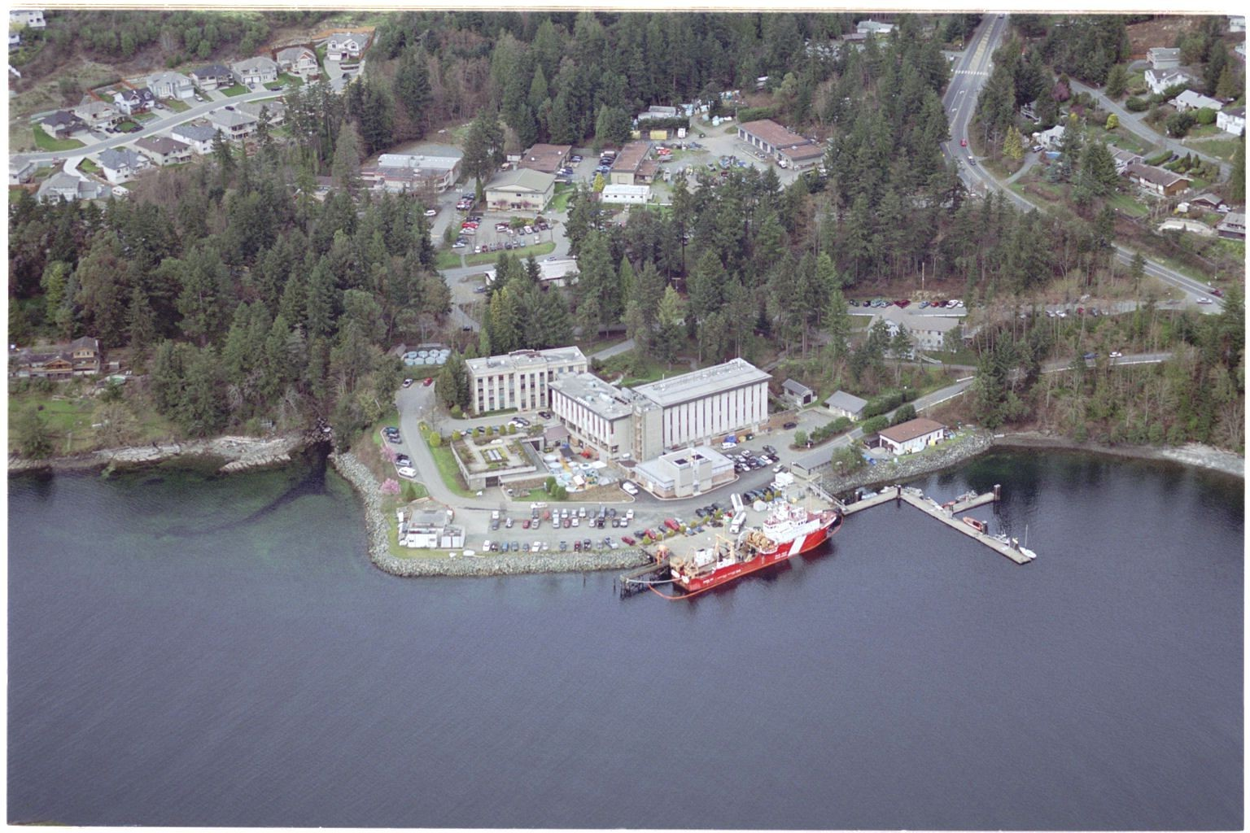
\includegraphics[height=3.5cm]{images/pbs.png}
  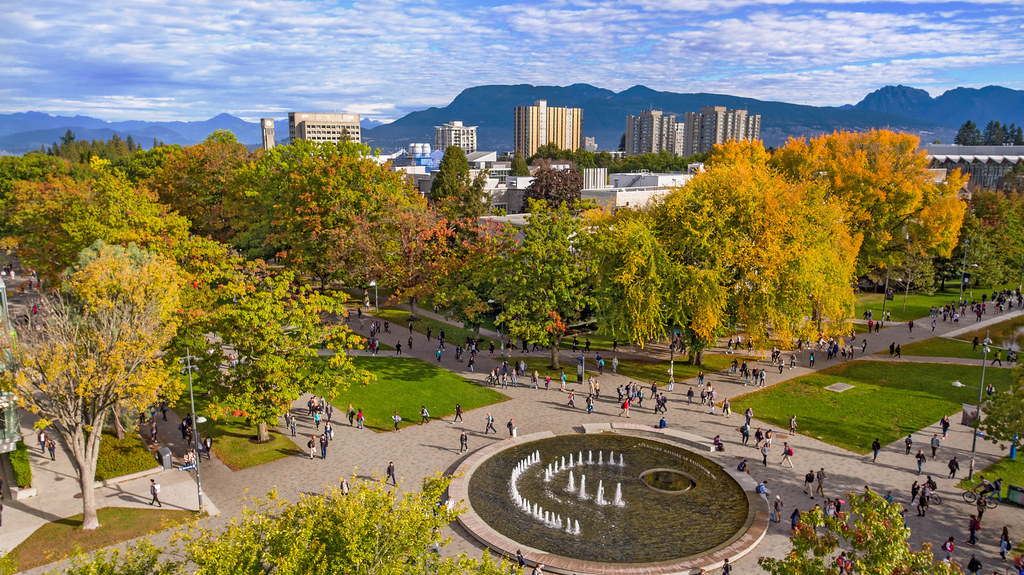
\includegraphics[height=3.5cm]{images/ubc-aerial.jpg}
  ~\\ \textcolor{blue}{$^1$Pacific Biological Station \& University of Victoria;
  $^2$University of British Columbia}}
% \institute{{\textcolor{blue}{Pacific Biological Station, Nanaimo, BC}\\
%  ~\\
% \institute{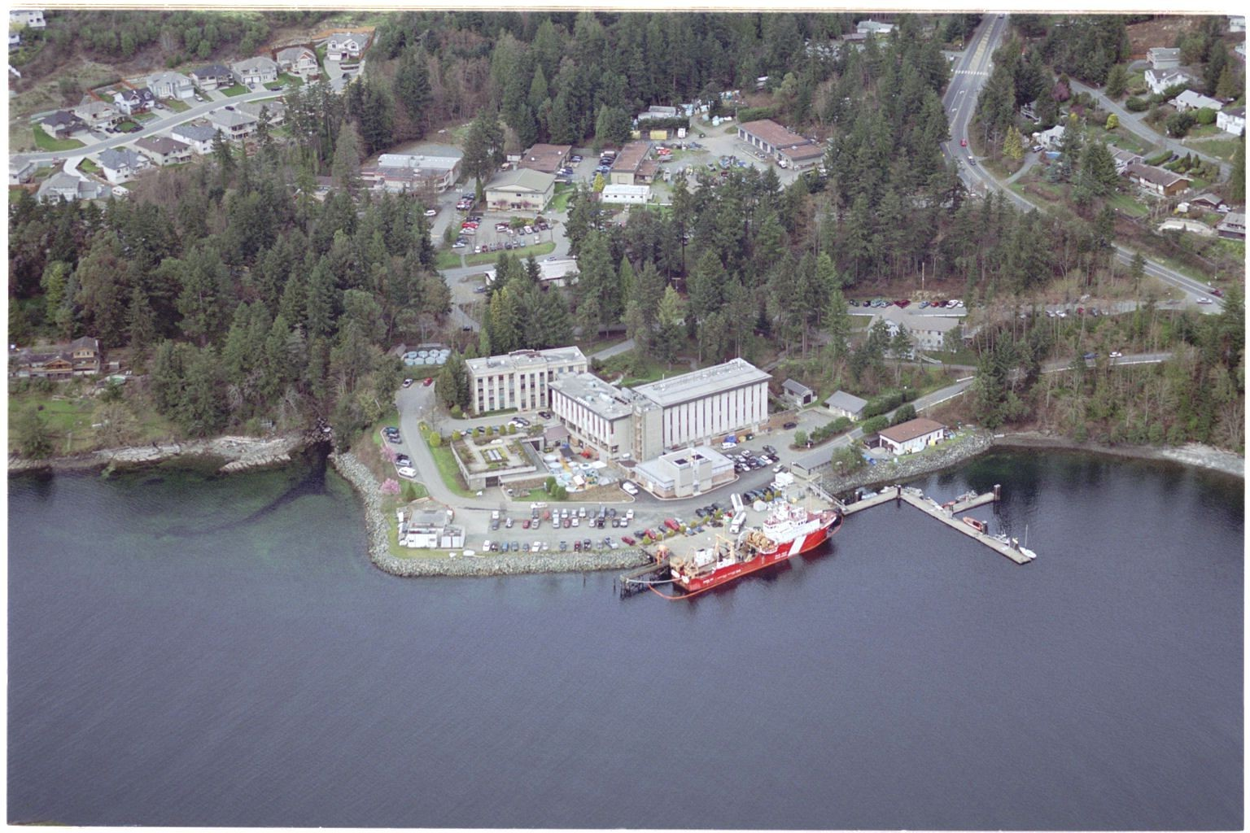
\includegraphics[height=3cm]{images/pbs.png}}
% \titlegraphic{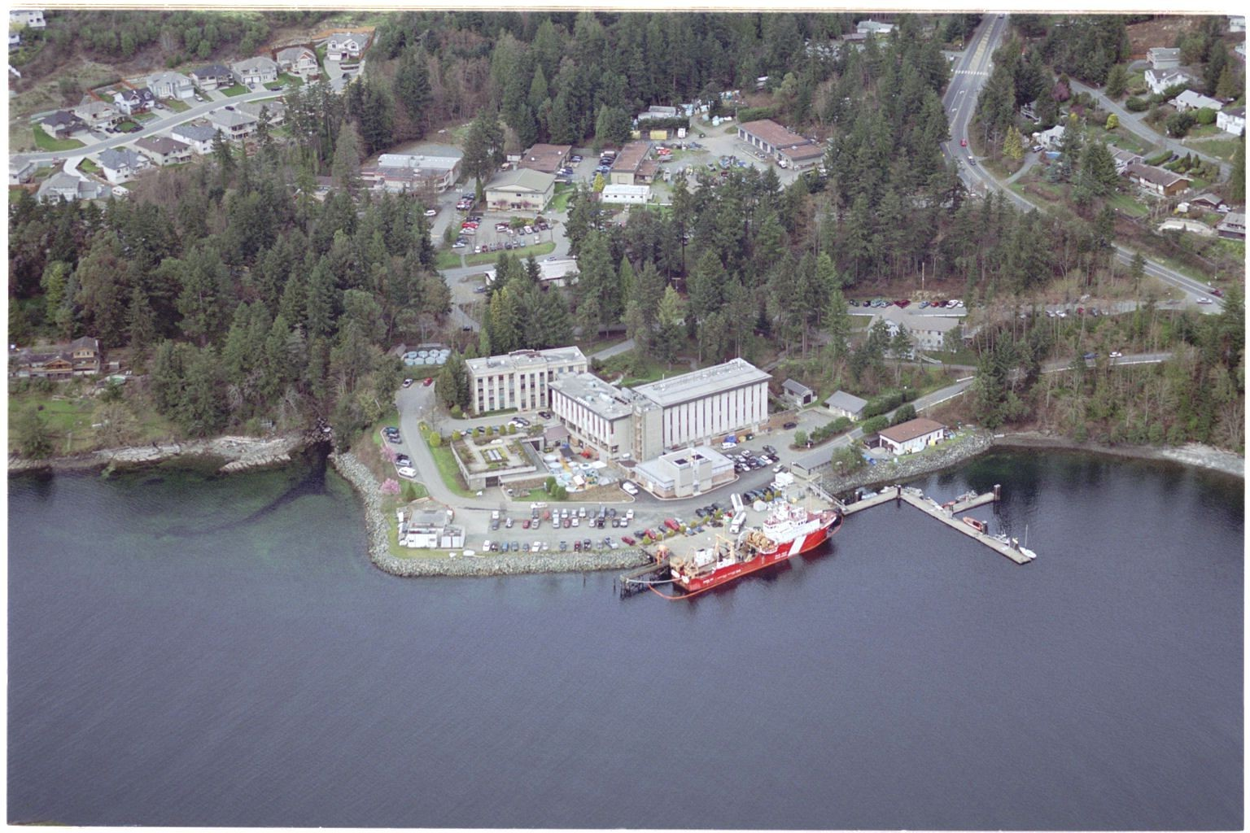
\includegraphics[height=3.3cm]{images/pbs.png}}
% \titlegraphic{images/pbs.png}
\date{{\footnotesize SRG meeting -- 2018}}
\subtitle{\small UVic Biology Department Seminar\\
Friday 1st November, 2019}
\IfFileExists{upquote.sty}{\usepackage{upquote}}{}

\setbeamertemplate{background}
{
\includegraphics[width=\paperwidth,height=\paperheight,keepaspectratio]{images/background-trans.png}}

\setbeamertemplate{itemize items}{
\includegraphics[scale=0.017]{images/halloween_pumpkin3.png}}
\setbeamertemplate{itemize subitem}{
\includegraphics[scale=0.017]{images/halloween_pumpkin2.png}}
\setbeamertemplate{itemize subsubitem}{
\includegraphics[scale=0.017]{images/halloween_pumpkin5.png}}

\newcommand{\eb}{\begin{eqnarray}}
\newcommand{\ee}{\end{eqnarray}}

\usefonttheme{serif}
\usepackage{mathptmx}    % Should have Times plus math fonts. AME used for Hake.
\usepackage{cancel}      % for \cancel (forget what the standard one is)

\begin{document}

\beamertemplatenavigationsymbolsempty   % bottom navigation panel
% \setbeamertemplate{headline}{}
% \setbeamertemplate{mini frames}{}

%\begin[plain]{frame}
\frame[plain]{
\titlepage
}
%----------------------------------------------------------

\setbeamertemplate{background}
{
\includegraphics[width=\paperwidth,height=\paperheight,keepaspectratio]{images/background-trans2.png}}
% fainter halloween picture for background

%----------------------------------------------------------

\begin{frame}
\frametitle{Paper}

%\begin{minipage}{6cm}
%Historical and projected spawning biomass for various catch levels
%\end{minipage}
%\begin{minipage}{6cm}
%\includegraphics[height=7.5cm]{images/projections.png}
%\end{minipage}

\begin{center}

\includegraphics[height=2.3cm]{images/mee-snip.png}
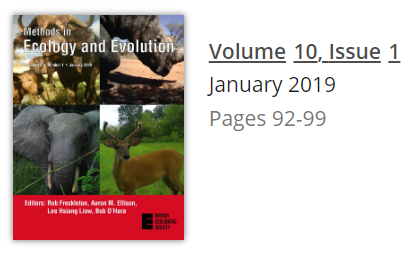
\includegraphics[height=2.3cm]{images/mee-snip-ref.png}\\
\end{center}

\rightline{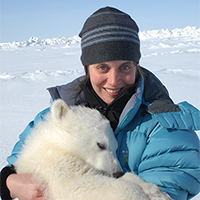
\includegraphics[height=2.3cm]{images/marie-polar-bear.jpg}}

\red{Code for building this talk: https://github.com/andrew-edwards/notation-talk}


\end{frame}

%----------------------------------------------------------

\begin{frame}
\frametitle{Feedback}

\centering
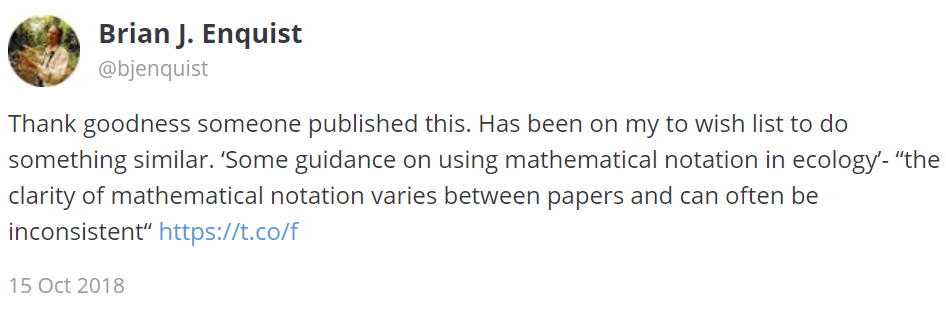
\includegraphics[height=2.6cm]{images/twitter-enquist.png}

\includegraphics[height=2.3cm]{images/twitter-miller.png}

\includegraphics[height=2.3cm]{images/twitter-oken.png}

\end{frame}

%----------------------------------------------------------

\begin{frame}
\frametitle{Feedback}

\centering

\includegraphics[height=2.3cm]{images/twitter-simpson.png}

\includegraphics[height=2.3cm]{images/twitter-tobias.png}

\includegraphics[height=2.3cm]{images/twitter-jonsen.png}

\end{frame}


%----------------------------------------------------------

\begin{frame}
\frametitle{Motivation}

We have both reviewed manuscripts in which unclear notation:
\bi
\item made it impossible to understand modelling details
\item \blue{meaning we could not evaluate the results or conclusions}
\item so could not properly review the work
\ei

\end{frame}

%----------------------------------------------------------


\begin{frame}
\frametitle{Motivation}
\bi
\item mathematical modelling playing an increasing role in biology
\item \blue{requires communication of details of models}
\item this includes notation
\item \blue{clarity of notation varies between papers}
\pause
\item poor notation can:
  \bi
  \item \red{make models appear more complicated than necessary}
  \item this leads to cluttered equations that impede understanding
  \item \red{impedes communication of ideas}
  \item can prevent work being properly reviewed -- analogous to an
      incomplete description of the methods of a laboratory experiment
  \ei
\ei
\end{frame}

% ----------------------------------------------------------

\begin{frame}
\frametitle{Motivation}
Lowry (1959) -- increase ``use of mathematical notation
where appropriate in ecological literature''.

TODO: figure:

equations in:
 14\% of the 37~contributions in the issue of \emph{Ecology} containing the
 Lowry (1959)

38\% of the 26~contributions comprising the March 2018 issue.
56\% of the 34~contributions in the March 2018 issue of \emph{Methods in Ecology and Evolution},

Lowry said advantages include:
\bi
\item precise communication of logical thought (beyond that afforded by
  the written word)
\item reproducibility of methods and results
\ei
and they ``accrue in proportion to
\red{the care used by the author in the use of notation}''.
\end{frame}

%----------------------------------------------------------

\begin{frame}
\frametitle{Motivation}
Many skills involved in producing ecological modelling paper, with books covering:
\bi
\item introductory ecology
\item general mathematics
\item ecological modelling
\item implementing models in R
\item writing and publishing a paper
\ei
  Recommendations exist for:
\bi
\item streamlining workflows (tools such as Git and GitHub)
\item making computer code available and reproducible
\ei
But no tips on developing the mathematical notation to use in a model.

\end{frame}

%----------------------------------------------------------

\begin{frame}
\frametitle{Motivation}

Improvements have impacts -- for Individual Based Models:

\bi
\item previously criticised as generally being so poorly documented
that they could not be evaluated or reproduced
\item motivated development of standardised protocols
\item led to a more rigorous formulation of models
\item enhanced understanding
\ei
\end{frame}

%----------------------------------------------------------

\begin{frame}
\frametitle{Motivation}

Why us?

\medskip

Similar backgrounds:
\bi
\item all research highly quantitative
\item \blue{lead authors of $>$20 ecological modelling papers}
\item taught modelling courses to biology students
\ei

\medskip
Differences:
\bi
\item one undergrad in math
\item \blue{one undergrad in biology}
\ei

\medskip

We have papers with notation that could, in hindsight, be improved.

\end{frame}


%----------------------------------------------------------

\begin{frame}
\frametitle{What is notation?}

\red{notation} -- we are specifically referring to:
\bi
\item letters used to represent quantities in equations
\item use of subscripts and superscripts
\item parentheses etc.
\item related concepts
\ei

Letters can be
\bi
\item Roman -- $a, b, c, ...$
\item Greek -- $\alpha, \beta, \gamma, ...$
\item lower case -- $a, b, c, \alpha, \beta, \gamma, ...$
\item upper case -- $A, B, C, \Gamma, \Delta, \Omega, ...$
\ei

\end{frame}

%----------------------------------------------------------

\begin{frame}
\frametitle{What do journals say?}
We reviewed the Author Guidelines for a sample of 14 journals:
\begin{multicols}{2}
\bi
\item \emph{Bulletin of Mathematical Biology}
\item \emph{Canadian Journal of Fisheries and Aquatic Sciences}
\item \emph{Ecology}
\item \emph{Ecology Letters}
\item \emph{Evolution$^*$}
\item \emph{Functional Ecology}
\item \emph{Journal of Animal Ecology}
\item \emph{Journal of the Royal Society Interface$^*$}
\item \emph{Marine Ecology Progress Series}
\item \emph{Methods in Ecology and Evolution}
\item \emph{Molecular Biology and Evolution}
\item \emph{Nature}
\item \emph{PLOS ONE}
\item \emph{Science}
\item[\vspace{\fill}]
\ei
\end{multicols}

$^*$Only two that have no mention of equations.

Minimal guidance in others -- almost exclusively restricted to typesetting aspects
(such as bold for vectors).

% rather than the broader considerations that we
%present here.
\end{frame}
%----------------------------------------------------------

\begin{frame}
\frametitle{Authors' responsibility}
Onus for good notation should be on authors (rather than journals)
because:
\bi
  \item notation should be decided early on in a study (possibly before deciding on a
    particular journal)
  \item ideally computer code will match the notation
  \item  work may first appear in a technical document such as a thesis before being
      submitted to a journal
  \item Supporting Information of a paper often contains the full mathematical details of
models and is not typeset or edited by publishers -- authors are responsible for
clarity
\ei
\end{frame}

%----------------------------------------------------------

\begin{frame}
\frametitle{Guidelines}
\bi
  \item based on those traditionally used in mathematics
  \item are in a somewhat logical order
  \item our aim is for them to be useful and adopted
  \item though we anticipate exceptions for which they are purposefully
    overlooked
  \item use examples from common ecological models, our own fields of research and from evolutionary biology
\ei
\end{frame}

%----------------------------------------------------------

\begin{frame}
\frametitle{1. Define all terms}

Who recognises this equation?
\eb
\nonumber E = mc^2
\ee

\pause Who knows what it means?

\medskip

\pause It does not convey any information, since the \red{letters are not
defined}.

\end{frame}

%----------------------------------------------------------

\begin{frame}
\frametitle{1. Define all terms}
Common ecological example:
\eb
\nonumber S = cA^z
\ee
\pause
where:
\bi
\item $S$ represents the number of species (of a particular taxonomic category)
in area $A$
\item constant $c$ is the
  number of species that would be in one square unit
\item dimensionless exponent $z$ quantifies the change in species number with area
\ei

\pause
So equation represents an increase in species richness with area.

\pause

\medskip

\blue{Immediately after an equation (as part of the same sentence)
any previously undefined symbols should be defined using the phrase}
\red{``where ...''}.
\end{frame}

%----------------------------------------------------------

\begin{frame}
\frametitle{1. Define all terms}

The number one guideline is to \red{define every term that is used in an equation}.

\pause

The number one guideline is to \red{define every term that is used in an equation}.

\pause

The number one guideline is to \red{define every term that is used in an equation}.

\pause

The number one guideline is to \red{define every term that is used in an equation}.

\pause

\medskip

Maybe introduce a second time if appears again much later in a lengthy work.

\medskip

\red{Table of notation} helpful for for complicated models.

\medskip

\pause

Desirable for tables and figures to be understandable on their own, so any
notation in them should be
additionally defined in their captions.


\end{frame}

%----------------------------------------------------------

% Sans serif fonts (like Arial) aren't great for math.

\begin{frame}
\frametitle{2. Use italics, boldface and capitalisation appropriately}

By convention, mathematical symbols (except Greek letters) should be italicised.

Distinguishes text from mathematical notation:

\bi
\item a large value of $a$
\item a large value of a
% \item much clearer in a serif font]
\ei

\pause

Vectors and matrices should be Roman script and bold:
\bi
\item {\bf a} is a vector
\item {\bf A} is a matrix
\item element $i$ of {\bf a} is often $a_i$
\item element in row $i$ and column $j$ of {\bf A} is  $A_{ij}$ (or sometimes
  $a_{ij}$)
\ei


Generic random variables are usually upper case:  $X$.

Possible numeric values represented by the corresponding lower-case letter: $x$.
\end{frame}

%----------------------------------------------------------


\begin{frame}
\frametitle{2. Use italics, boldface and capitalisation appropriately}

Roman letters for standard mathematical functions:
\bi
\item $\sin x$, $\cos x$, $\log x$, $\ln x$, e$^x$
\ei
and for other words such as:
\eb
\nonumber X \sim \mbox{Normal}(\mu, \sigma^2)
\label{Xnormal}
\ee
\pause
for variable $X$ coming from a normal distribution with mean $\mu$ and
standard deviation $\sigma$.
\pause

\medskip
Also use a Roman d for derivative and integral of variable $X$ with respect to time $t$:
\eb
\nonumber \frac{\mbox{d}X}{\mbox{d}t} ~~~~~~\mbox{and}~~~~~~ \int f(x) \mbox{d}x
\ee

\pause
\medskip

Units should be given in Roman type to distinguish them from mathematical variables:
\bi
\item the speed of the polar bear was 1~km~h$^{-1}$
\item let the speed be $x$~km~h$^{-1}$
\ei

\end{frame}

%----------------------------------------------------------

\begin{frame}
\frametitle{3. Use subscripts appropriately}

Subscripts represent different values of a quantity.

\bi
\item $B_t$ -- biomass of a population in year $t$, where
$t=1, 2, 3, ..., T$, and $T$ is the maximum year.
\ei

\pause

\red{Cannot} then use:

\bi
\item $B_s$ -- biomass in spatial area $s$, where $s=1, 2, 3, ..., S$, and $S$
  is the number of areas.
  \ei

\pause

Because:

\bi
\item $t=1$ gives $B_1$ as the biomass in year 1

\item $s=1$ also gives $B_1$ as the biomass in spatial area 1
\ei

Obvious confusion.

\end{frame}

%----------------------------------------------------------

\begin{frame}
\frametitle{3. Use subscripts appropriately}

Should use:

\bi
\item $B_{st}$ -- biomass in area $s$ in year $t$ (for various combinations of $s$ and $t$)
\ei

\pause

Extending this, for data from fish trawl surveys:
\bi
  \item $B_{ijkmn}$ -- biomass caught per hour (g~h$^{-1}$) of:
  \bi
    \item taxonomic group $i$
    \item length class $j$
    \item haul $k$
    \item by vessel $m$
    \item in year $n$
  \ei
\ei

Succinctly describes detailed structure of the data, and made subsequent
calculations unambiguous.

\pause
\medskip

\red{Commas:} can use $B_{st}$ or $B_{s,t}$, but always use them to avoid
ambiguity: $B_{3,17}$ rather than $B_{317}$.

\end{frame}

%----------------------------------------------------------

\begin{frame}
\frametitle{3. Use subscripts appropriately}

Abbreviations as (non-italicised) subscripts to indicate related
definitions.

\medskip

For example, when modelling DNA records from sediments:
\bi
  \item $P_\mathrm{fp}$ -- probability of {\bf f}alse {\bf p}ositives
  \item $P_\mathrm{fn}$ -- probability of {\bf f}alse {\bf n}egatives
\ei
\pause
\medskip

Fisheries:
\bi
  \item $B_\mathrm{MSY}$ -- biomass of a stock at the maximum sustainable yield (MSY)
\ei
So MSY is not an index (like $B_t$), but an acronym that is non-italicised to
distinguish from the related $B_t$.
\pause
\medskip

Please please please avoid using acronyms such as $MSY$ to represent a variable.

\end{frame}

%----------------------------------------------------------

\begin{frame}
\frametitle{3. Use subscripts appropriately}

Usually, a subscript as an index should appear on both sides of
an equation:
\eb
\nonumber y_t = 2 x_t + 3,
\ee
for the relationship between two variables $x_t$ and $y_t$ at each time $t$.
% there is a value of $y_t$ corresponding to each setting of $t$.

\pause

Should generally \red{not} be a mixture of subscripts:
\eb
\nonumber y_t = 2 x_i + 3.
\ee

% Else $y_t$ depends on the value of $x_i$, and therefore on $i$.

\medskip

Can lead to confusion:
\bi
  \item $i = 1, x_1 = 3$ gives $y_t = 9$
  \item $i = 2, x_2 = 5$ gives $y_t = 13$
\ei
Should use $y_{it}$.

\pause

An expression such as
\eb
\nonumber y_{ij} = 2 x_i + 3
\ee
is valid.
%-- it just means that the $ij$ value of $y$ is the same
%for all values of the index $j$ (since nothing on the right-hand side depends
%n $j$).

\end{frame}

%----------------------------------------------------------

\begin{frame}
\frametitle{3. Use subscripts appropriately}

\red{Source of confusion:} $i$ and $j$ as indices, but using one again in a summation:
\eb
\nonumber y_{\textcolor<2->{blue}{i}j} = 2 x_{\textcolor<2->{blue}{i}j} +
  \sum_{\textcolor<3->{red}{i}=1}^N x_{\textcolor<3->{red}{i}j}
\ee

\bi
  \item \onslide<2-> $\blue{i}$ used on both sides here as an index (equation valid for all values
    of $\blue{i}$)
  \item \onslide<3-> $\red{i}$ used in summation as a dummy index
\ei

\onslide<4->
Solution: use $k$ as a dummy index:
\eb
\nonumber y_{ij} = 2 x_{ij} + \sum_{\red{k}=1}^N x_{\red{k}j}
\ee

\onslide<5->
Another way to understand:
\eb
\nonumber \sum_{\red{k}=1}^N x_{\red{k}j} = \sum_{\red{l}=1}^N x_{\red{l}j} = \sum_{\red{m}=1}^N x_{\red{m}j}
\ee
since $\red{k}, \red{l}$ and $\red{m}$ are just dummy indices.

\end{frame}

% Skipping: For spatio-temporal situations, an alternative to the aforementioned $B_{st}$
% is using $Y_t(s)$ ....

%----------------------------------------------------------

\begin{frame}
\frametitle{4. Be careful with superscripts}

Superscripts can distinguish related variables:
\bi
  \item $X$
  \item $X'$
\ei

Though be careful -- single quotes sometimes used for derivatives of functions:
\bi
\item $f'(x)$
\ei
or transpose of vectors and matrices:
\bi
\item $\mathbf{X}'$
\ei
but transpose can also be
\bi
  \item $\mathbf{X}^{\mbox{t}}$
  \item $\mathbf{X}^{\mbox{T}}$
\ei

Asterisks traditionally represent the steady state of a dynamic variable:
\bi
  \item $X^*$
\ei

\end{frame}

%----------------------------------------------------------

\begin{frame}
\frametitle{4. Be careful with superscripts}

Please please please \red{do not use} a number or a letter (as an index) as a
superscript:
\bi
  \item $B^t$ -- biomass in year $t$
\ei
but this looks like $B$ raised to the power $t$.

Setting $t=2$ gives
\bi
  \item $B^2$
\ei
which is interpreted as $B \times B$, not the desired biomass in year~2.

\pause

Even worse example:
\bi
  \item $u_{at}^{sg}$ -- exploitation rate of fish of:
  \bi
    \item sex $s$
    \item age $a$
    \item caught by fishing gear $g$
    \item in year $t$
  \ei
\ei

Just use subscripts and go with
\bi
  \item $u_{atsg}$
\ei
like the earlier example of $B_{ijkmn}$.
\end{frame}

%----------------------------------------------------------

\begin{frame}
\frametitle{4. Be careful with superscripts}
Subscripts and superscripts should always come after the variable. Not:
\bi
  \item $_jv_t$
\ei

Otherwise, if $\theta$ multiplied by $_jv_t$ gives
\bi
  \item $\theta_jv_t$
\ei
but ambiguous: is first component $\theta_j$ or $\theta$?


\end{frame}

%----------------------------------------------------------

\begin{frame}
\frametitle{5. Helpful to distinguish variables from parameters}

Example -- Ricker model:
\eb
\nonumber R = \alpha S \mbox{e}^{-\beta S}
\label{ricker}
\ee
where
\bi
  \item $R$ -- the recruitment of new fish (dependent variable on the left-hand
    side)
  \item $S$ -- the spawning stock biomass (independent variable on the right-hand
    side)
  \item $\alpha$ -- maximum number of recruits produced by each unit
  of spawning stock biomass (parameter)
  \item $\beta$ -- scales the intensity of density dependence (parameter).
\ei

% The model says how the variables $R$ and $S$ relate to each other.
% Using particular parameter values of $\alpha$ and $\beta$ distinguishes one
% realisation of the model from another.

\end{frame}

%----------------------------------------------------------

\begin{frame}
\frametitle{5. Helpful to distinguish variables from parameters}

\eb
\nonumber R = \alpha S \mbox{e}^{-\beta S}
\label{ricker}
\ee

The model says how the variables $R$ and $S$ relate to each other.

\medskip

Using particular parameter values of $\alpha$ and $\beta$ distinguishes one
realisation of the model from another:

\centering
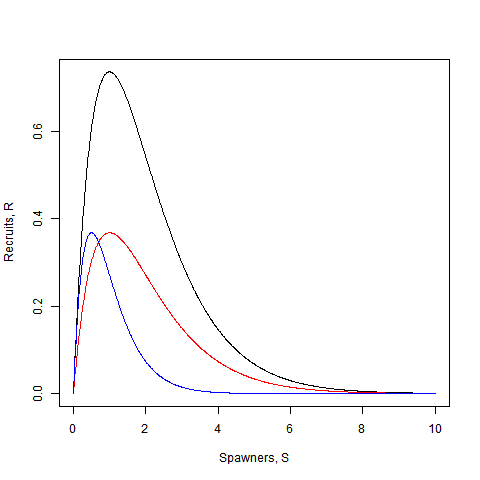
\includegraphics[height=4cm]{images/ricker.png}

\end{frame}



%----------------------------------------------------------

\begin{frame}
\frametitle{5. Helpful to distinguish variables from parameters}

Useful, if possible:
\bi
 \item variables -- upper case
 \item parameter and constants (like gravitational constant $g$) -- lower case
   and Greek letters
\ei

However, stick with established convention when this is not followed, or for
simple equations such as
\eb
\nonumber y = 3 x + 7
\ee
with variables $x$ and $y$ (often the first choice to represent variables).

\end{frame}

%----------------------------------------------------------

\begin{frame}
\frametitle{Quiz time}

\centering
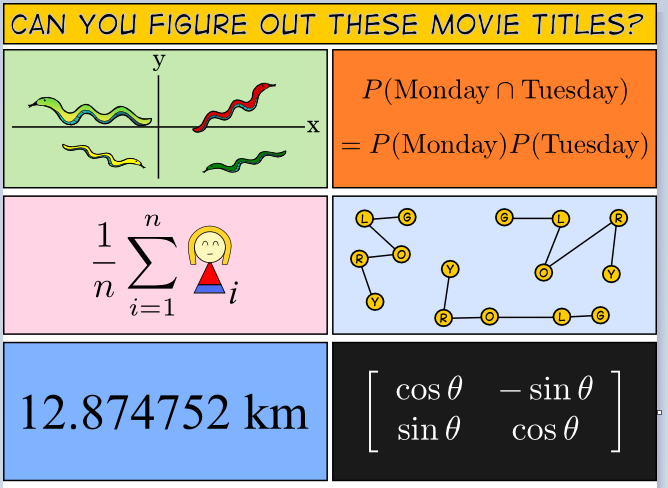
\includegraphics[height=6cm]{images/movies2.png}\\

\includegraphics[height=0.5cm]{images/movies-credit.png}

\end{frame}

%----------------------------------------------------------

\begin{frame}
\frametitle{6. Avoid multi-letter variable names}

Use only \red{one letter} (rather than two or more) to represent a quantity.

Common abbreviation: SSB for spawning stock biomass.

Fine as an \red{acronym in a sentence}, but problematic when $SSB$ used as a
mathematical quantity in an equation:

\bi
  \item $SSB_t$ -- spawning stock biomass in year $t$
  \item $S$ -- selectivity (proportion of biomass caught by fishing)
  \item $B_t$ -- total (spawning plus non-spawning) biomass in year $t$
\ei

But this breeds ambiguity:
% \onslide<1>{S}\onslide<2>{\red{S}}  ~~~~\alt<1>{hello}{goodbye}  - latter worked
\eb
\nonumber \frac{S B_t}{SSB_t} \onslide<2->{= \frac{\cancel{S}
    B_t}{\cancel{S}SB_t}}
  \onslide<3->{= \frac{S \cancel{B_t}}{SS\cancel{B_t}}}\onslide<2->{~~~~~~?}
\ee
\pause

% \frac{\alt<1>{S}{\cancel{\red{S}}} B_t}{SSB_t}
% \alt<1>{\frac{S B_t}{SSB_t}}{\frac{\cancel{\red{S}} B_t}{SSB_t}
% \alt<1>{\frac{a}{b}}{\frac{c}{d}}
  % ~~~~~~~~~~{\textcolor<2->{red}{?}
% ~~~~~~~~~~{\textcolor<2->{red}{?}
% \nonumber \frac{\onslide<1>{S} \onslide<2>{\red{S}} B_t}{SSB_t}

\onslide<4>Solution: pick, say, $B_t$ and $T_t$ for, respectively, the spawning and total biomasses at time $t$.

\end{frame}

%----------------------------------------------------------

\begin{frame}
\frametitle{6. Avoid multi-letter variable names}

Occasionally may be okay to use an acronym or word as a variable name.

Often used in simple statistical models:
\eb
\nonumber \mbox{e}^{\beta_1 + \beta_2 \times \mbox{MeanDepth}_i}
\ee
which intuitively represents an exponential effect of a linear
function of mean depth ($\beta_1$ and $\beta_2$ are parameters).

\pause

\bi
  \item such statistical models generally require no further subsequent mathematical
  manipulation
  \item may avoid the problems outlined in previous slide
\ei

\pause

Words or acronyms can make models more understandable:
\bi
\item e.g. for stakeholders who are not quantitatively trained
\item for a presentation or a poster, especially if not all details of
  a model are going to be given
  \ei

\pause

Just ensure:
\bi
  \item no potential for confusion (can be hard to guarantee when
    first defining notation)
  \item equations don't become cumbersome and hard to understand
\ei

\end{frame}

%----------------------------------------------------------

\begin{frame}
\frametitle{6. Avoid multi-letter variable names}

One solution is to simultaneously give equations in word and notation form:

\centering

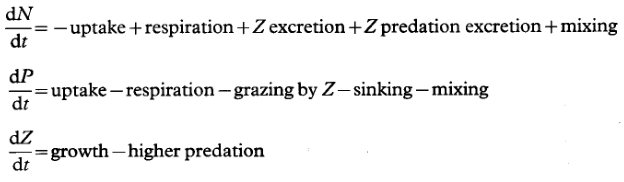
\includegraphics[height=2cm]{images/eb96-words.png}\\
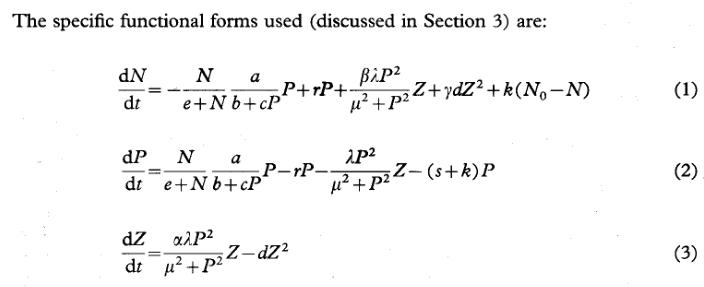
\includegraphics[height=2.8cm]{images/eb96-eqns.png}


\end{frame}

%----------------------------------------------------------

\begin{frame}
\frametitle{7. Fully define probability distributions}

\bi
\item \red{Discrete} random variable -- takes discrete values (e.g.~1, 2, 3, ...)
\ei

$f(x)$ -- \emph{probability mass function} of a \red{discrete} variable $X$:
\eb
\nonumber f(x) = \mbox{P}(X = x)
\ee
where % Is the probability that $X$ takes each possible value of $x$, i.e.~
\bi
\item P$(\cdot)$ -- probability of occurrence of the event in parentheses ($X$
  takes the value $x$)
\ei

\medskip

For example, Poisson distribution for count data:
\eb
\nonumber f(x) = \frac{\lambda^x \mbox{e}^{-\lambda}}{x!}, ~~ x = 0, 1, 2, ...
\ee
where $x$ are the possible values and there is just one parameter $\lambda>0$.

\end{frame}

%----------------------------------------------------------

\begin{frame}
\frametitle{7. Fully define probability distributions}

\bi
\item \blue{Continuous} random variable -- can take any value within a specified range
  (e.g.~between 0 and 10).
\ei

$f(x)$ -- \blue{continuous} probability density function, for example:
\eb
\nonumber f(x) = \frac{1}{\sqrt{2 \pi} \sigma x} \mbox{e}^{-(\log x - \mu)^2 / 2
  \sigma^2}, ~~ x > 0
\ee
for parameters $\mu$ and $\sigma$, and $\log$ is \red{natural logarithm}.

\medskip

Worth defining `$\log$' and using $\log_{10}$ for
base-10 logarithm (realising $\ln$ is also used for the natural logarithm).


\end{frame}

%----------------------------------------------------------


\begin{frame}
\frametitle{7. Fully define probability distributions}

Note in both examples the \red{domain} is specified:
\eb
\nonumber f(x) & = & \frac{\lambda^x \mbox{e}^{-\lambda}}{x!}, ~~ \red{x = 0, 1, 2,
  ...}\\
\nonumber f(x) & = & \frac{1}{\sqrt{2 \pi} \sigma x} \mbox{e}^{-(\log x - \mu)^2 / 2
  \sigma^2}, ~~\red{x > 0}
\ee

This also helps confirm the distribution is appropriate for the
question at hand.

\medskip

\pause

Normal distribution -- generally no need to explicitly specify that
$-\infty < x < \infty$.

\end{frame}

%----------------------------------------------------------

\begin{frame}
\frametitle{7. Fully define probability distributions}

For \red{discrete} and \blue{continuous} distributions, can define
\bi
\item $F(x)$ -- cumulative probability distribution:
\ei

\eb
\nonumber \mbox{\red{discrete}} ~~~~~ F(x) & = & \mbox{P}(X \leq x) =
\sum_{i=0}^{x} f(i)\\
\nonumber  & & \\
\nonumber \mbox{\blue{continuous}} ~~~~~F(x) & = & \mbox{P}(X \leq x) = \int_{- \infty}^x f(u) \mbox{d}u
\ee

\end{frame}

%----------------------------------------------------------


\begin{frame}
\frametitle{7. Fully define probability distributions}

For a second random variable, $Y$, possible options are:
\bi
\item $g(y)$
\item $f_Y(y)$,  and use $f_X(x)$ for $X$
\item $f(y)$ -- does \red{not} work as \red{not distinguishable} from $f(x)$
\ei

\pause

Some distributions have a conventional shorthand, e.g.:
\bi
\item $X \sim \mbox{N}(\mu, \sigma^2)$ -- variable $X$ is normally distributed with
  mean $\mu$ and standard deviation $\sigma$
\item $X \sim \mbox{N}(0,2)$ -- here specify whether the 2 is the standard
  deviation or the variance to avoid ambiguity
\item $X \sim \mbox{Gamma}(a, b)$ -- Gamma distribution, but define parameters
  as can be parameterised using shape and either rate, scale or mean
\ei

\end{frame}

%----------------------------------------------------------


\begin{frame}
\frametitle{8. Give equations of a model rather than just computer code}

One reason that acronyms or words get used to identify variables may be
that this is how they are written in computer code.

\medskip

Words in code can make code easier to read and avoid typographical errors.

\medskip
But words in equations are not recommended. Solutions:
\bi
\item write equations first and then have a comment in the corresponding code that links the words used in the code to the
  corresponding mathematical notation
\item \red{modern simpler alternative is the R~package {\tt knitr}}
\item {\tt knitr} interweaves text and computer code in a
  single file, easily enabling the same succinct notation to be used throughout
\item \red{{\tt Rmarkdown} now allows easy interweaving math, code, write up, references,
  figures etc.}
\ei

\end{frame}

%----------------------------------------------------------


\begin{frame}
\frametitle{8. Give equations of a model rather than just computer code}

\bi
\item Writing equations may seem a necessary prerequisite to writing code
\item Some people are proficient programmers but are sometimes unable to translate the
  code into mathematical notation
\ei

For example, for a numeric vector {\tt x} in R, the command
\eb
\nonumber {\tt y <\!\!\!- ~ cumsum(x)}
\ee
is defined as creating a vector {\tt y} where each element is the cumulative sum
of the elements of {\tt x}.

Equivalent math: for a vector ${\bf x}$ of length $n$,
\eb
\nonumber y_i = \sum_{j=1}^i x_j, ~~~ i=1, 2, 3, ..., n.
\ee

\pause
However, the verbal description is ambiguous, unlike the equation.


\end{frame}

%----------------------------------------------------------


\begin{frame}
\frametitle{8. Give equations of a model rather than just computer code}

The {\tt cumsum(x)} example is usually just for book-keeping.

\medskip

But for more complex code (e.g. log-likelihood functions), give the equation not
the code, since:
\bi
\item code relies on reader having knowledge of that particular language
\item languages evolve and fall out of favour
\item properly documented equations will stand the test of time
\item useful to supply code as Supporting Information or as a package
\ei

\end{frame}

%----------------------------------------------------------

\begin{frame}
\frametitle{9. Abide by conventions (but still define everything)}

\centering Common mathematical usage of particular letters and symbols
\begin{table}
  \centering\rowcolors{2}{gray!6}{white}
  \begin{tabular}{ll}
\hline
Letter/symbol & Common usage\\
\hline
$e$ & usually avoided to prevent confusion with non-italicised e ($=$2.718...)\\
  % base of natural logarithm,
$f, g$ & function, e.g.~$f(x) = x^3 + 7$\\
$i, j, k$ & index, e.g.~the $i$th element of vector {\bf x} is $x_i$\\
$n, N$ & sample size\\
$o, O$ & usually avoided to prevent confusion with number 0\\
$t$ & time\\
$u, v, w$ & speeds\\
$x, y, z$ & variables, or co-ordinates in space\\
\mbox{P}$(\cdot)$ & probability of occurrence of the event in parentheses\\
$X, Y, Z$ & variables\\
\hline
\end{tabular}
\rowcolors{2}{white}{white}
\end{table}

\end{frame}

%----------------------------------------------------------

\begin{frame}
\frametitle{9. Abide by conventions (but still define everything)}

\centering Common mathematical usage of particular letters and symbols
\begin{table}
  \centering\rowcolors{2}{gray!6}{white}
  \begin{tabular}{ll}
\hline
Letter/symbol & Common usage\\
\hline
$\alpha, \beta, \gamma, \theta$ & parameters\\
$\delta, \Delta$ & difference or change in a variable, $\Delta X$, or a
  parameter\\
$\epsilon$ & a small value, or random noise term\\
$\mu$ & mean\\
$\pi$ & the value 3.141...\\
$\prod$ & product of the proceeding values\\
$\sigma$ & standard deviation\\
$\sum$ & summation of the proceeding values\\
$X^*$ & steady-state value of $X$\\
$\dot{X}$ & derivative of $X$\\  % also $x'$ but that's really just physicists
$f'(x)$ & derivative of $f(x)$ with respect to $x$\\
$\partial f/\partial x$ & partial derivative of $f(x,y)$ with respect to $x$\\
$\hat{\theta}$ & an estimate of $\theta$\\
\hline
\end{tabular}
\rowcolors{2}{white}{white}
\end{table}

\end{frame}

%----------------------------------------------------------

\begin{frame}
\frametitle{9. Abide by conventions (but still define everything)}

Compare:

1. The population size is given by
\eb
\nonumber  t_\epsilon = g t_{\epsilon-1} (1 - t_{\epsilon-1}) + f_\epsilon
\label{screwy}
\ee
where
\bi
\item $t_\epsilon$ -- population in year $\epsilon$ ($\epsilon = 1, 2, 3, ...,
  \Gamma$)
\item $g$ -- intrinsic growth rate at low population size
\item  $f_\epsilon$ -- normally distributed random noise with mean $\sigma$ and variance $\mu^2$
\ei

\end{frame}

%----------------------------------------------------------

\begin{frame}
\frametitle{9. Abide by conventions (but still define everything)}

2. The population size is given by
\eb
\nonumber X_t = r X_{t-1} (1 - X_{t-1}) + \epsilon_t
\label{sensible}
\ee
where
\bi
\item $X_t$ -- population in year $t$ ($t = 1, 2, 3, ..., T$)
\item $r$ -- intrinsic growth rate at low population size
\item $\epsilon_t$ -- normally distributed random noise with mean $\mu$ and variance $\sigma^2$.
  \ei

\end{frame}

%----------------------------------------------------------

\begin{frame}
\frametitle{9. Abide by conventions (but still define everything)}

Within some fields, certain notation may be standard.

\medskip

But still clearly define notation, in particular because
of the multidisciplinary nature of ecology.


\medskip

Established conventions:
\bi
\item may be best to try to retain
\item but maybe not if conventional notation was not well thought-out
\item can help when learning a new area
\item multidisciplinary work -- can be hard to retain all conventions (and
  appease everyone)
  \ei

\end{frame}

%----------------------------------------------------------

\begin{frame}
\frametitle{Quiz time}

\centering
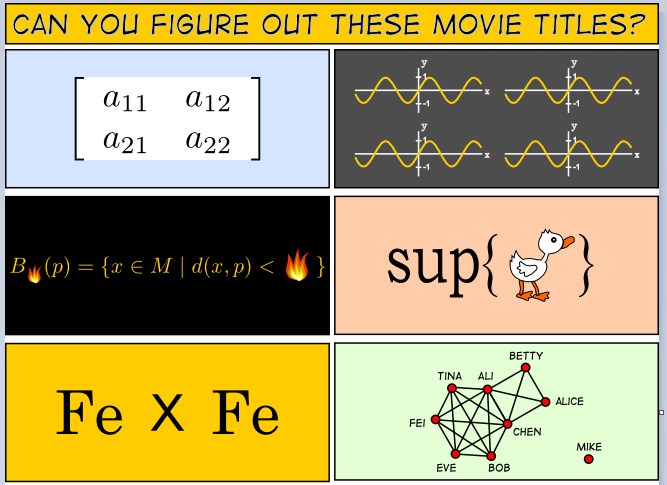
\includegraphics[height=6cm]{images/movies1.png}\\

\includegraphics[height=0.5cm]{images/movies-credit.png}

\end{frame}


%----------------------------------------------------------

\begin{frame}
\frametitle{10. Use parentheses and brackets only as necessary}

Parentheses $()$
\bi
\item around the arguments of a function, e.g.~$f(x)$
\item denote which calculations in an equation need to be done first, e.g. $3 (x
  + 5)$
\ei

To avoid too many  many slightly-different sized parentheses also use:
\bi
\item square brackets $[~]$
\item braces $\{\}$
\ei

\pause

But don't overuse parentheses:
\eb
\nonumber f(x) = \frac{\left(\lambda^x\right) \left(\mbox{e}^{-\lambda}\right)}{x!},
  ~~ x = 0, 1, 2, ...
\ee
makes the equation appear more complicated than it is.

% We have seen happen
This often happens in practice -- but extra clutter can impede comprehension.

\end{frame}

%----------------------------------------------------------

\begin{frame}
\frametitle{10. Use parentheses and brackets only as necessary}

Almost always no need to use a symbol such as $\times$ or $\cdot$ for
multiplication, unless
\bi
\item using words as variable names
\item breaking up long equations for readability
\ei

\pause

Parentheses also used:
\bi
\item $x \in (0, 1)$ means $0 < x < 1$
\item $x \in [0, 1]$ means $0 \leq x \leq 1$
\item $x \in [0, 1)$ means $0 \leq x < 1$
\ei

\end{frame}

%----------------------------------------------------------

\begin{frame}
\frametitle{11. Equations should be part of sentences}

Sometimes require punctuation:
\bi
\item maybe a comma when in middle of sentence
\item a period when completing a sentence
\ei

\pause

Worth numbering all equations, (even if not referred to later):
\bi
\item easier for others to refer to
\item easier for your future self to refer to
\ei

\pause

\medskip

Single terms in equations (or very simple equations) appear within
text and not on their own line.

\medskip

Fractions within such lines should be $a/b$ not $\frac{a}{b}$.

\end{frame}

%----------------------------------------------------------

\begin{frame}
\frametitle{12. Revise notation early on if necessary}

\bi
\item Think about notation before defining a model
\item Can be useful to revisit notation \emph{early on} in a project once some
  details are fleshed out
\item But hard to change notation once proceeded far enough, such as:
  \bi
  \item two papers already published
  \item thousands of lines of computer code shared with others
    \bi
  \item potentially confusing to switch notation in related works
    \ei
    \ei
\ei

Thus, time spent revisiting notation early on may be time well spent.

\pause

\medskip

Similar to functionalising computer code -- taking a
pause and rewriting code in a more user-friendly way tends to pay off in future.

\end{frame}

%----------------------------------------------------------

\begin{frame}
\frametitle{12. Revise notation early on if necessary}

Related point -- PROOFREAD. % mention K&H paper

\medskip

Different publishers have different minor typsetting rules (that may or may not
impact comprehension).

\medskip

Letters should have unique definition in single piece of work.

\end{frame}

%----------------------------------------------------------

\begin{frame}
\frametitle{Example of confusing notation}

Highlights several problems:
\eb
\nonumber \sigma_a^{\textcolor<2,4>{red}{s}^2} = \left( \frac{{\textcolor<3>{blue}{sd}}^{\textcolor<2,4>{red}{S}}_a}{L^{\textcolor<2,4>{red}{S}}_a} \right)^2
\ee
where:
\bi
\item ${\textcolor<3>{blue}{sd}}^{\textcolor<2,4>{red}{S}}_a$  -- standard deviation of the length of a fish of age $a$ and sex
  $\textcolor<4>{red}{S}$
\item $\sigma_a^{\textcolor<2,4>{red}{s}}$ -- standard deviation of the distribution of log(length) at
  age $a$ for sex $\textcolor<4>{red}{s}$
\item $L^{\textcolor<2,4>{red}{S}}_a$ -- length at age $a$ for sex $\textcolor<4>{red}{s}$
\item $\textcolor<4>{red}{s}$ -- sex, $\textcolor<4>{red}{s}=1$ for females and $\textcolor<4>{red}{s}=2$ for males
\ei

\end{frame}

% ----------------------------------------------------------

\begin{frame}
\frametitle{Closing remarks}

Hope these guidelines:
\bi
\item are useful
\item help improve future comprehension of biological models
\item help improve reproducibility
\ei

\medskip

Re-iterate: these are \red{guidelines} but \red{not rules}, and should be overlooked when appropriate.

\bigskip

\medskip

{\bf Acknowledgements}

Jaclyn Cleary,
Brooke Davis,
Wayne Hajas,
James Robinson,
Catarina Wor,
Brianna Wright.

Three anonymous reviewers, Sean McMahon and Robert O'Hara.

\end{frame}

%----------------------------------------------------------

\end{document}

% ----------------------------------------------------------

\begin{frame}
\frametitle{}

\end{frame}

%----------------------------------------------------------

% ----------------------------------------------------------

\begin{frame}
\frametitle{}

\end{frame}

%----------------------------------------------------------

% ----------------------------------------------------------

\begin{frame}
\frametitle{}

\end{frame}

%----------------------------------------------------------

% notation-rev.tex: take some bits to put into talk, delete un-needed:


\section*{Author contributions} AE conceived the idea for this work
and then AE and MAM wrote it together.
% Both authors contributed critically to the drafts and gave final approval for publication.

\section*{Data accessibility}

This work uses no data.

\bibliography{notation}

\clearpage

\thispagestyle{empty}

% Do captions this way if manuscript accepted.
% Table \ref{tab:letters} caption.

% Caption text....

% \clearpage

% \renewcommand{\arraystretch}{1.9}  % forces table double spaced


\begin{frame}
\frametitle{}
\bi
  \item
\ei
\end{frame}

%----------------------------------------------------------
The use of a superscript $s$ to index sex requires another higher-level
superscript in the term $\sigma_a^{s^2}$ to denote that the standard deviation
term $\sigma_a^s$ is being squared. The $sd$ on the right-hand side stands for
standard deviation (one letter would suffice, especially with $s$ being used
elsewhere), and the superscript $S$ is capitalised on the right-hand side but not
on the left. Equation (\ref{sigma2}) is simply scaling a standard deviation by
a length value, but looks much more complicated than that due to the choice
of notation.
